%-------------------------------------------------------------------------------
%-------------------------------------------------------------------------------
%-------------------------------------------------------------------------------
\insertTitle{Планирование и анализ эксперимента}{1}{ПМ-63}{Кожекин М.В.}{Майер В.А.}{Назарова Т.А.}{Утюганов Д.С.}{9(1)}{2020}


%-------------------------------------------------------------------------------
\section{Цель работы}
Изучить понятие оптимального плана эксперимента и критерии оптимальности планов.


%-------------------------------------------------------------------------------
\section{Задание}

1.	Изучить понятия непрерывного плана эксперимента и информационной матрицы, а также критерии оптимальности, связанные с точностью оценивания параметров модели и точностью оценивания математического ожидания функции отклика.

2.	Разработать программу по обработке различных планов эксперимента для регрессионных моделей. Обработка заключается в вычислении различных характеристик плана, связанных с тем или иным критерием оптимальности.

3.	Для каждого из планов вычислить значения функционалов от информационной (дисперсионной) матриц, связанных с такими критериями, как: $D-$, $A-$, $E-$, $\Phi_2-$, $\Lambda-$,  $MV-$, $G-$ оптимальности. Проранжировать планы, указанные в варианте, с позиций различных критериев. Выбрать план, наиболее предпочтительный по совокупности критериев. Список планов приведен в табл. 1.

4.	В качестве спектра плана выбрать один из приведенных в табл. 1 для соответствующей модели. Веса точек выразить в виде зависимости от одного параметра, как в примере аналитического построения оптимального плана. Для этого параметра определить допустимые интервалы значений, руководствуясь тем, что веса точек должны быть неотрицательные, а число таких точек с ненулевыми весами должно быть не меньше числа параметров в модели. Построить графики изменения критерия оптимальности плана, указанного в варианте, в зависимости от этого скалярного параметра; определить по графику оптимальные значения параметра и критерия. Сравнить полученный результат с результатами из п. 3.

5.	Оформить отчет, включающий в себя постановку задачи, полученные результаты и текст программы.

6.	Защитить лабораторную работу. 


%-------------------------------------------------------------------------------
\section{Анализ}

В рамках работы исследуется общая линейная модель:
\[ y = f^T(x)\Theta + \varepsilon = \sum_{l=1}^m f_l(x)\Theta_l + \varepsilon \]
\[ y = \Theta_0 + \Theta_1 \cdot x + \Theta_2 \cdot x^2 \]

Исходя из варианта задания (1) эксперимент проводится в трёх точках -1, 0, 1

{\bf Непрерывным нормированным планом} эксперимента называется совокупность величин вида

\[
	\varepsilon^*=
	\begin{bmatrix}
	    x_1		&	x_2		&	\cdots		&	x_n	\\
 	    p_1		&	p_2		&	\cdots		&	p_n
	\end{bmatrix}
	\text{где } \sum_{i=1}^n p_i = 1, p_i \geq 0
\] 

{\bf Информационной матрицей} дискретного непрерывного плана называется величина
\[M = \sum_{j=1}^n p_j f(x_j)f^T(x_j) = \frac{X^T X}{N}\]

Матрица, обратная к информационной, называется {\bf дисперсионной}
\[ D(\varepsilon)=M^{-1}(\varepsilon) D(\varepsilon_N)=M^{-1}(\varepsilon_N) \]

Критерии оптимальности плана эксперимента:
\[ D-\text{оптимальности } \varepsilon^* = Arg \min_{\varepsilon} |D(\varepsilon)| \]
\[ A-\text{оптимальности } \varepsilon^* = Arg \min_{\varepsilon} tr D(\varepsilon) \]
\[ E-\text{оптимальности } \varepsilon^* = Arg \min_{\varepsilon} \max_i \lambda_i[D(\varepsilon)] \]
\[ \Phi_2-\text{оптимальности } \varepsilon^* = Arg \min_{\varepsilon} \sqrt{m^{-1} tr D^2(\varepsilon)} \]
\[ \Lambda-\text{оптимальности } \varepsilon^* = Arg \min_{\varepsilon} \sum_{i=1}^n [ \lambda_j(D(\varepsilon)) - \overline{\lambda}(D(\varepsilon)) ]^2 \]
\[ MV-\text{оптимальности } \varepsilon^* = Arg \min_{\varepsilon} \max_i D_{ii}(\varepsilon) \]
\[ G-\text{оптимальности } \varepsilon^* = Arg \min_{\varepsilon} \max_{x \in \hat{X}} d(x, \varepsilon) \]
\[ d(x, \varepsilon) = f^T(x) M^{-1} f(x) \]


%-------------------------------------------------------------------------------
\section{Выбор оптимального плана}

В каждом из 4 вариантов эксперимент проводится в трёх точках: -1, 0, 1

\( y = \Theta_0 + \Theta_1 \cdot x + \Theta_2 \cdot x^2 \)

\begin{tabular}{|c|c|c|c|}
\hline
	№ & $p_1$ & $p_2$ & $p_3$ \\ 
\hline
	1 & 0.2 & 0.6 & 0.2 \\ 
	2 & 0.25 & 0.5 & 0.25 \\ 
	3 & 0.1884 & 0.6233 & 0.1884 \\ 
	4 & 0.333 & 0.333 & 0.333 \\
\hline
\end{tabular}

Найдём информационные и дисперсионные матрицы для каждого из вариантов:

{\bf Матрицы M:}

\begin{tabular}{|c|c|c|c|}
\hline
	variant 1 & variant 2 & variant 3 & variant 4 \\ 
\hline
\begin{tabular}{ccc}
 1.0 &  0.0 &  0.4 \\
 0.0 &  0.4 &  0.0 \\
 0.4 &  0.0 &  0.4 \\
\end{tabular} &
\begin{tabular}{ccc}
 1.0 &  0.0 &  0.5 \\
 0.0 &  0.5 &  0.0 \\
 0.5 &  0.0 &  0.5 \\
\end{tabular} &
\begin{tabular}{ccc}
 1.00 &  0.00 &  0.38 \\
 0.00 &  0.38 &  0.00 \\
 0.38 &  0.00 &  0.38 \\
\end{tabular} &
\begin{tabular}{ccc}
 1.00 &  0.00 &  0.67 \\
 0.00 &  0.67 &  0.00 \\
 0.67 &  0.00 &  0.67 \\
\end{tabular} \\ 
\hline
\end{tabular}

{\bf Матрицы D:}

\begin{tabular}{|c|c|c|c|}
\hline
	variant 1 & variant 2 & variant 3 & variant 4 \\ 
\hline
\begin{tabular}{ccc}
 1.67 &  0.0 & -1.67 \\
 0.00 &  2.5 &  0.00 \\
-1.67 &  0.0 &  4.17 \\
\end{tabular} &
\begin{tabular}{ccc}
 2.0 &  0.0 & -2.0 \\
 0.0 &  2.0 &  0.0 \\
-2.0 &  0.0 &  4.0 \\
\end{tabular} &
\begin{tabular}{ccc}
 1.6 &  0.00 & -1.60 \\
 0.0 &  2.65 &  0.00 \\
-1.6 &  0.00 &  4.26 \\
\end{tabular} &
\begin{tabular}{ccc}
 3.0 &  0.0 & -3.0 \\
 0.0 &  1.5 &  0.0 \\
-3.0 &  0.0 &  4.5 \\
\end{tabular} \\ 
\hline
\end{tabular}

\begin{tabular}{rrrrrrrrrrrrrr}
\toprule
 \multicolumn{2}{l}{D} & \multicolumn{2}{l}{A} & \multicolumn{2}{l}{E} & \multicolumn{2}{l}{Phi\_2} & \multicolumn{2}{l}{Lambda} & \multicolumn{2}{l}{MV} & \multicolumn{2}{l}{G} \\
 i &  value &  i & value &  i & value &     i & value &      i &  value &  i & value &  i & value \\
\midrule
 4 &   6.77 &  2 &  8.00 &  1 &  5.00 &     2 &  2.83 &      3 &   8.72 &  2 &  4.00 &  2 &  4.00 \\
 2 &   8.00 &  1 &  8.33 &  3 &  5.01 &     1 &  2.97 &      1 &   8.80 &  1 &  4.17 &  1 &  4.17 \\
 1 &  10.42 &  3 &  8.52 &  2 &  5.24 &     3 &  3.04 &      2 &  10.67 &  3 &  4.26 &  3 &  4.26 \\
 3 &  11.30 &  4 &  9.01 &  4 &  6.85 &     4 &  3.24 &      4 &  22.55 &  4 &  4.50 &  4 &  4.50 \\
\bottomrule
\end{tabular}


Исходя из совокупности критериев оптимальным является план из варианта 2.

\[
	\varepsilon^*= \begin{bmatrix}
	-1		&	0		&	1		\\
	0.25	&	0.5		&	0.25
	\end{bmatrix}
\] 


%-------------------------------------------------------------------------------
\section{Выбор оптимального параметра}

Под планом понимается модель из варианта 4 вида:

\[
	\varepsilon^*=
	\begin{bmatrix}
	    -1		& 		 0		 & 		1		\\
 	     q		& 1 - 2\cdot q &		q
	\end{bmatrix}
	q \in (0, 0.5)
\] 


\begin{figure}[!htb] %htbp!
	\centering
	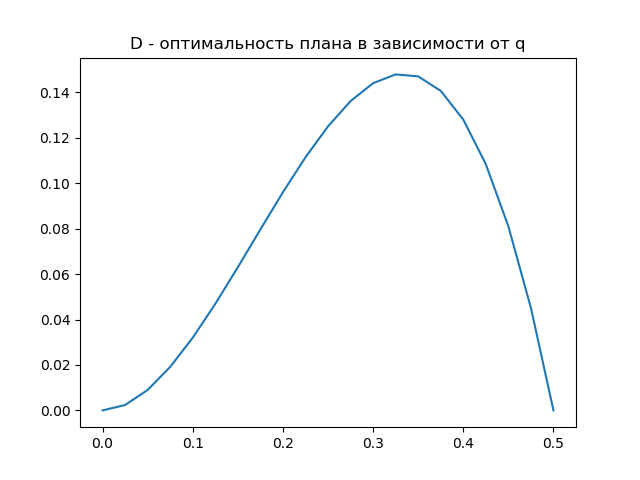
\includegraphics[width=0.5\textwidth]{opt_q.png}
	\caption{Оптимальное значение параметра q = 0.333}
\end{figure}


Проверим решение аналитически:

\[
	M = q \cdot
	\begin{bmatrix}
		 1		\\
		-1		\\
		 1
	\end{bmatrix}
	\cdot
	\begin{bmatrix}
	    1 & -1 & 1
	\end{bmatrix}
	+ (1 - 2\cdot q) \cdot
	\begin{bmatrix}
		1		\\
		0		\\
		0
	\end{bmatrix}
	\cdot
	\begin{bmatrix}
	    1 & 0 & 0
	\end{bmatrix}
	+ q \cdot
	\begin{bmatrix}
		1		\\
		1		\\
		1
	\end{bmatrix}
	\cdot
	\begin{bmatrix}
	    1 & 1 & 1
	\end{bmatrix}
\]


\[
	M = q \cdot
	\begin{bmatrix}
		 1		&	 -1		&		1	\\
		-1		&	  1		&     -1	\\
		 1		&	 -1		&		1
	\end{bmatrix}
	+ (1 - 2\cdot q) \cdot
	\begin{bmatrix}
		 1		&	  0		&		0	\\
		 0		&	  0		&      0	\\
		 0		&	  0		&		0
	\end{bmatrix}
	+ q \cdot
	\begin{bmatrix}
		 1		&	  1		&		1	\\
		 1		&	  1		&      1	\\
		 1		&	  1		&		1
	\end{bmatrix}
\]

\[
	det(M) =
	\begin{bmatrix}
		 1		&	  0		&	   2q	\\
		 0		&	 2q		&		0	\\
		2q		&	  0		&	   2q
	\end{bmatrix}
	= 4q^2 + 0 + 0 - 8q^3 - 0 - 0
	= 4q^2 - 8q^3
\]
\[ \frac{d(|M|)}{dq} = 4 \cdot 2 q - 8 \cdot 3 q^2 = 0 \]
\[ \frac{d(|M|)}{dq} = 3 q^2 - q = 0 \]
\[ \text{Аналитическое значение параметра } q = \frac{1}{3} \]


%-------------------------------------------------------------------------------
\section{Исходный код программы}
\myCodeInput{python}{lab1.py}{../lab1.py}